\providecommand{\pgfsyspdfmark}[3]{}

\documentclass[11pt,letterpaper]{article}
\usepackage[lmargin=1in,rmargin=1in,tmargin=1in,bmargin=1in]{geometry}

% -------------------
% Packages
% -------------------
\usepackage{
	amsmath,			% Math Environments
	amssymb,			% Extended Symbols
	enumerate,		    % Enumerate Environments
	graphicx,			% Include Images
	lastpage,			% Reference Lastpage
	multicol,			% Use Multi-columns
	multirow,			% Use Multi-rows
	gensymb
}


% -------------------
% Font
% -------------------
\usepackage[T1]{fontenc}
\usepackage{charter}
\usepackage{xcolor}

% -------------------
% Commands
% -------------------

\newcommand{\prob}{\noindent\textbf{Problem. }}
\newcounter{problem}
\newcommand{\problem}{
	\stepcounter{problem}%
	\noindent \textbf{Problem \theproblem. }%
}
\newcommand{\answer}{\noindent \textbf{Answer. }}
\newcommand{\pspace}{\par\vspace{\baselineskip}}
\newcommand{\ds}{\displaystyle}


% -------------------
% Header & Footer
% -------------------
\usepackage{fancyhdr}

\fancypagestyle{pages}{
	%Headers
	\fancyhead[L]{}
	\fancyhead[C]{}
	\fancyhead[R]{}
\renewcommand{\headrulewidth}{0pt}
	%Footers
	\fancyfoot[L]{}
	\fancyfoot[C]{}
	\fancyfoot[R]{}
\renewcommand{\footrulewidth}{0.0pt}
}
\headheight=0pt
\footskip=14pt

\pagestyle{pages}


% -------------------
% Content
% -------------------
\begin{document}
\noindent\textbf{\large Calculus I (AM\_\_1050AH / MSF\_10110) \\ 2022 Fall \\ Application of Derivatives (5.2-5.3) (Answer Key)}

\bigskip

\noindent Note that in problems for related rates, you should clearly indicate the unit of your answer. 

\bigskip

\problem Let $f(x) = x^2 - 10x + 9$,
\begin{enumerate}[(a)]
    \item Find the roots of $f(x)$ using factorization.
    \item Find the roots of $f(x)$ using Newton's method, with initial guess set as $10$ and tolerance set at $10^{-5}$.  How many iterations was needed to reach tolerance?
    \item Find the roots of $f(x)$ using Newton's method, with initial guess set as $6$ and tolerance set at $10^{-5}$.  How many iterations was needed to reach tolerance?
    \item Compare the number of iteration in (b) and (c) and provide an explanation for their difference.
\end{enumerate}\vspace{6mm}

\answer Since subproblems (b) and (c) involves Newton's method, we first derive the formula for each iteration, which involves the first derivative $f'(x) = 2x-10$: if the $k^{\text{th}}$ guess of the root is $x_k$, then the $(k+1)^{\text{th}}$ guess $x_{k+1}$ is given by:
\[x_{k+1} = x_k - \frac{f(x_k)}{f'(x_k)} = x_k - \frac{x_k^2-10x_k+9}{2x_k-10}\]
\begin{enumerate}[(a)]
    \item Using factorization, we have $f(x) = x^2 - 10x + 9 = (x-1)(x-9)$.  Therefore, there are two roots for $f(x)$, $1$ and $9$.
    \item The iterations are as follows, which requires $3$ iteration steps (stopping for $0.00000152 < 10^{-5}$).
    \begin{center}
        \begin{tabular}{ccc}
            Iteration ($k$) & $x_k$ & $f(x_k)$ \\
            \hline
            $0$ & $10$ & $9$\\
            $1$ & $10-\frac{9}{2 \cdot 10 - 10} = 9.1$ & $0.81$\\
            $2$ & $9.1 - \frac{0.81}{2 \cdot 9.1 - 10} \approx 9.00121951$ & $0.00975757$\\
            $3$ & $9.00121951 - \frac{0.00975757}{2 \cdot 9.00121951 - 10} \approx 9.00000019$ & $0.00000152$
        \end{tabular}    
    \end{center}
    \item The iterations are as follows, which requires $5$ iteration steps (stopping for $0.00000512 < 10^{-5}$).
    \begin{center}
        \begin{tabular}{ccc}
            Iteration ($k$) & $x_k$ & $f(x_k)$ \\
            \hline
            $0$ & $6$ & $-15$\\
            $1$ & $6-\frac{-15}{2 \cdot 6 - 10} = 13.5$ & $56.25$\\
            $2$ & $13.5 - \frac{56.25}{2 \cdot 13.5 - 10} \approx 10.19117647$ & $10.94831314$\\
            $3$ & $10.19117647 - \frac{10.94831314}{2 \cdot 10.19117647 - 10} \approx 9.13666472$ & $1.11199501$\\
            $4$ & $9.13666472 - \frac{1.11199501}{2 \cdot 9.13666472 - 10} \approx 9.00225752$ & $0.01806526$\\
            $5$ & $9.00225752 - \frac{0.01806526}{2 \cdot 9.00225752 - 10} \approx 9.00000064$ & $0.00000512$
        \end{tabular}    
    \end{center}
    \item (b) requires less iterations since its initial guess ($10$) is closer to the root ($9$) than (c)'s initial guess ($6$).
\end{enumerate}\vspace{6mm}


\noindent\begin{minipage}{0.7\textwidth}
    \problem A kid is holding a balloon with a string of length $150$ centimeters, and the balloon is now of height $90$ centimeters, shown in the graph on the right. Suppose the string is always taut, and the balloon is floating upwards with its height increasing by $15$ cm per second.  At what rate is the angle $\theta$ increasing?
\end{minipage}
\begin{minipage}{0.3\textwidth}
    \begin{center}
        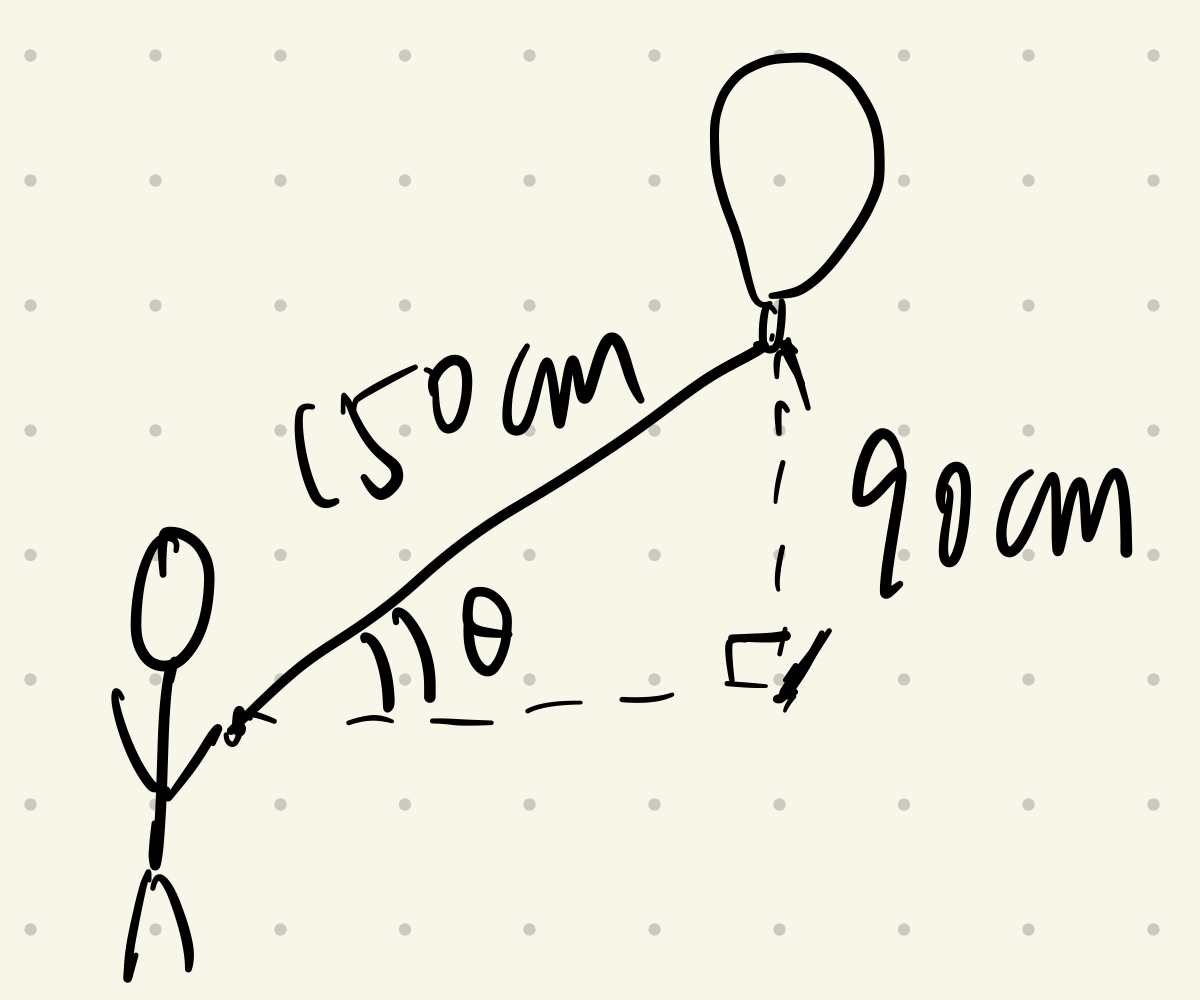
\includegraphics[width = 0.8\textwidth]{../graph/A11.png}
    \end{center}
\end{minipage}
\vspace{12mm}

\answer Denote the height of the balloon as $h$ cm, then at any given time, we have 
    \[150 \sin \theta = h\]
    Differentiating both sides by time $t$ (in seconds) and denoting $()'$ as differentiation by $t$:
    \[150 (\sin \theta)' = h' \qquad \Rightarrow \qquad 150 (\cos \theta) \theta' = h' \]
    where we applied chain rule on the left side, differentiating by $\theta$ first.  
    
    Currently $h = 90$, so we have $\sin \theta = \frac{90}{150} = \frac{3}{5}$, therefore currently $\cos \theta = \frac{4}{5}$.  Furthermore, $h$ is currently increasing by $15$ per second, i.e. $h' = 15$,  so we yield the current rate of change of $\theta$:
    \[\theta' = \frac{h'}{150 \cos \theta} = \frac{15}{150\cdot\frac{4}{5}} = \frac{1}{8}\]
    Therefore, the angle $\theta$ is increasing at a rate of $\frac{1}{8}$ radians per second.
\begin{center}
    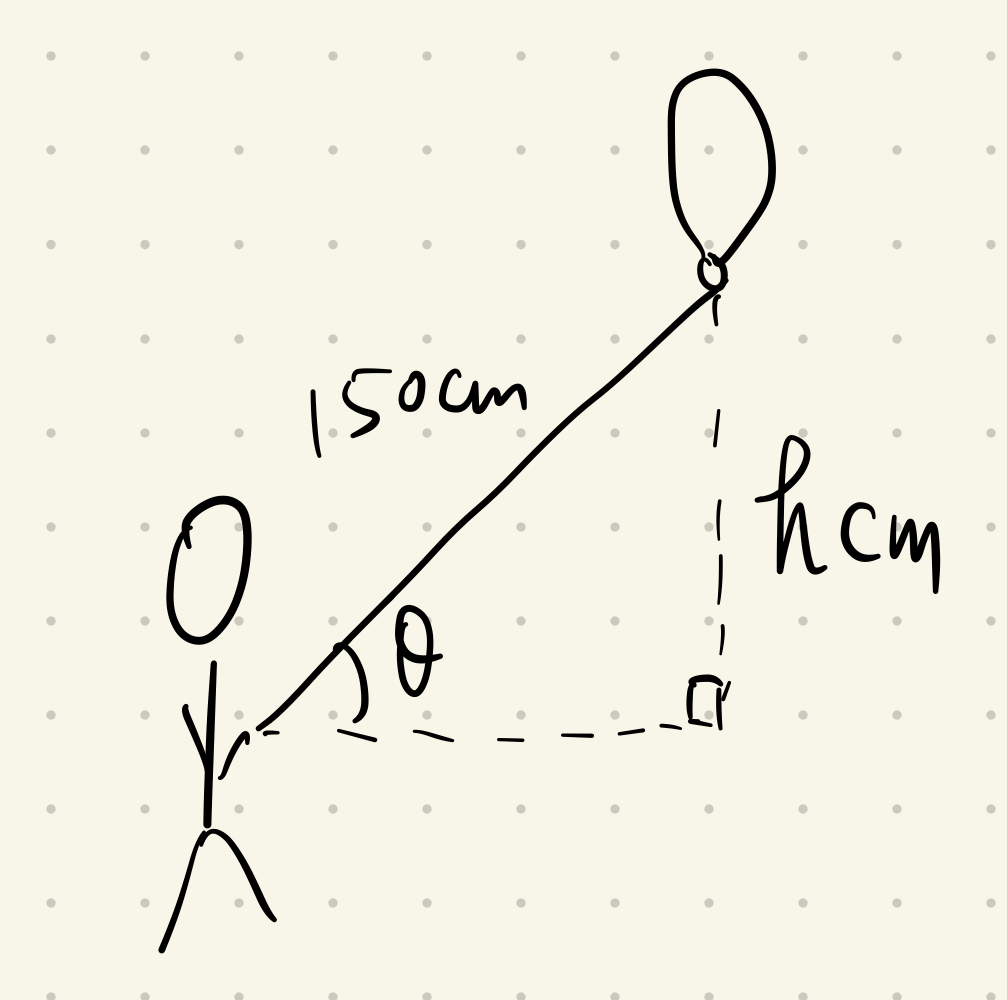
\includegraphics[width = 0.25\textwidth]{../graph/A11_Sol_1.png}
\end{center}\vspace{6mm}

\problem A sake bottle shaped like a cone is of radius $7$ cm at the bottom with height $10.5$ cm,
\begin{enumerate}[(a)]
    \item It is known that the volume of a cone with radius $r$ at the bottom and height $h$ is $\frac{1}{3}\pi r^2 h$.  Calculate the amount of sake in the bottle when the fluid level is $X$ cm from the bottom.
    \item Suppose we are pouring sake into the bottle at a constant speed of $30 \pi \approx 94.25$ cc/seconds.  If the current fluid level is just $3$ cm from the bottom, how fast is the fluid level rising now?
    \item From (b), if the current fluid level is $9$ cm from the bottom instead, how fast is the fluid level rising now?
\end{enumerate}\vspace{6mm}

\pagebreak

\answer 

\begin{figure}[h]
    \centering
    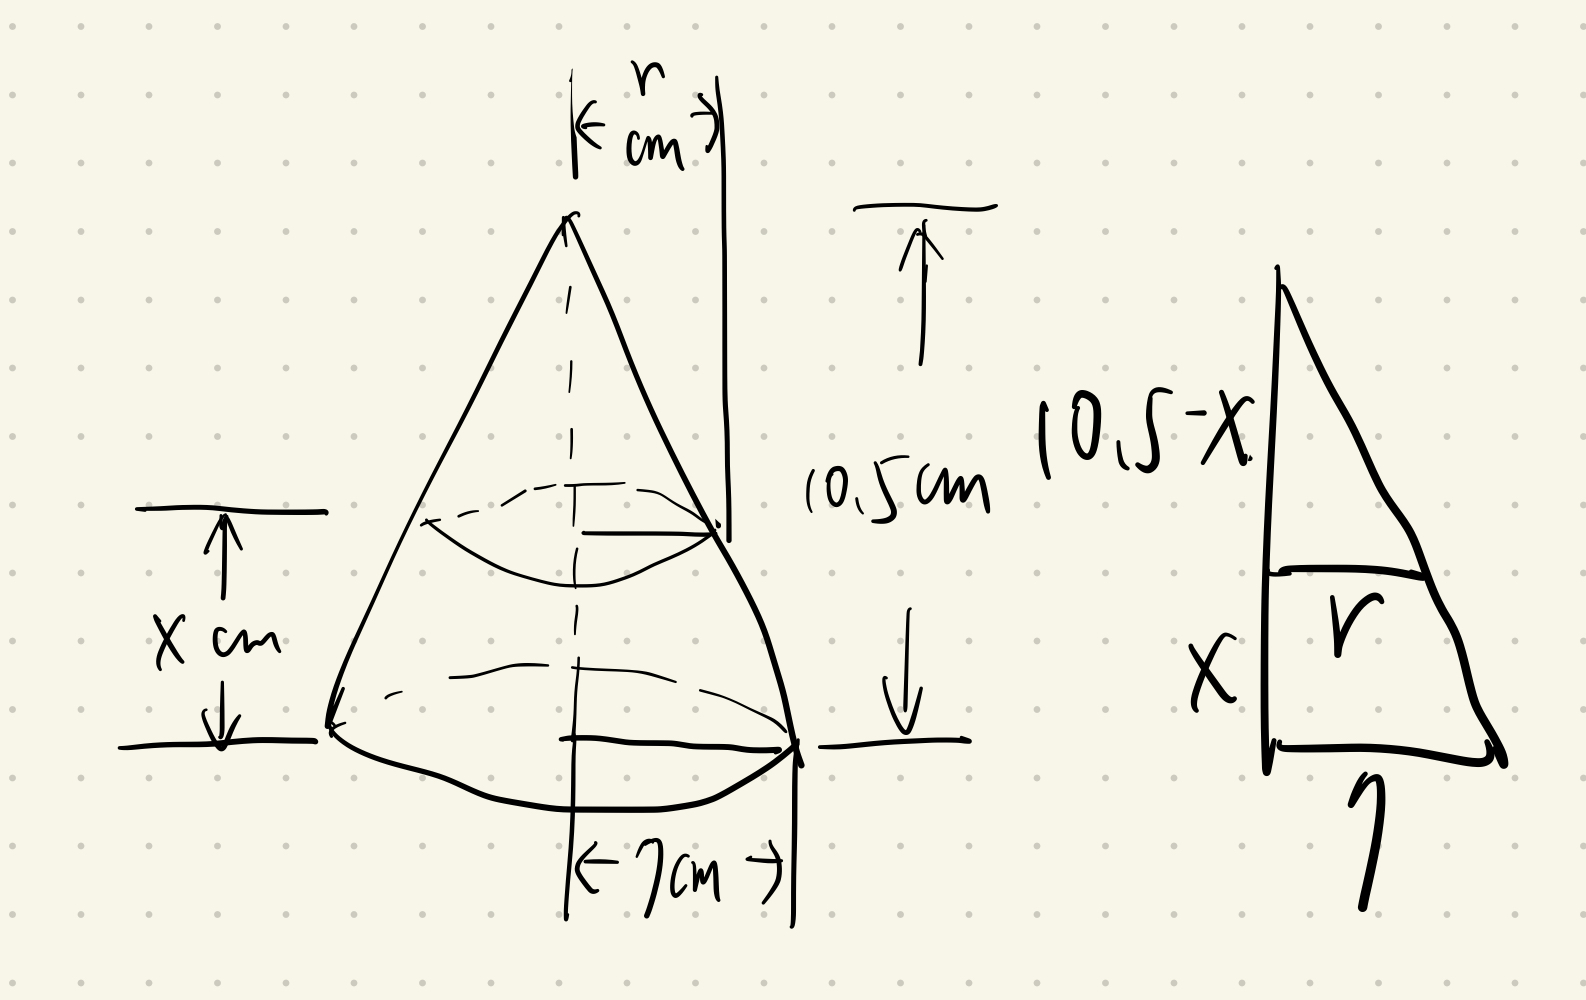
\includegraphics[width = 0.5\textwidth]{../graph/A11_Sol_2.png}
\end{figure}

\begin{enumerate}[(a)]
    \item The volume of the sake, as shown in the figure above, is the difference between the entire volume of the cone-shaped bottle and the upper cone without the sake.  The volume of the whole bottle, from the formula for the volume of cones, is $\frac{1}{3}\pi \cdot 7^2 \cdot 10.5$.  To calculate the volume of the upper cone, we need to derive the radius of its bottom, shown as $r$ in the figure.  Using the similar triangles on the right, we have:
    \[\frac{10.5-X}{r} = \frac{10.5}{7} \quad \Rightarrow r = \frac{7}{10.5}(10.5-X) = 7-\frac{7}{10.5}X = 7-\frac{2}{3}X\]
    Therefore, the volume of the upper cone is $\frac{1}{3}\pi r^2 (10.5-x) = \frac{1}{3}\pi(7-\frac{2}{3}X)^2(10.5-X)$, and the volume of the sake can be calculated as:
    \begin{align*}
        \frac{1}{3}\pi \cdot 7^2 \cdot 10.5-\frac{1}{3}\pi\Big(7-\frac{2}{3}X\Big)^2(10.5-X) &= \frac{1}{3}\pi \cdot 7^2 \cdot 7 \cdot \frac{3}{2} -\frac{1}{3}\pi\Big(7-\frac{2}{3}X\Big)^2\Big(7 \cdot\frac{3}{2}-X\Big)\\
        &= \frac{\pi}{2}\cdot 7^3 - \frac{\pi}{3}\Big(7-\frac{2}{3}X\Big)^2\Big(7-\frac{2}{3}X\Big)\cdot \frac{3}{2}\\
        &= \frac{\pi}{2}\cdot 7^3 - \frac{\pi}{2}\Big(7-\frac{2}{3}X\Big)^3 = \frac{\pi}{2}\Big[7^3 - \Big(7-\frac{2}{3}X\Big)^3\Big]
    \end{align*}
    So the volume of the sake given fluid level of $X$ cm from the bottom is $\frac{\pi}{2}\big[7^3 - \big(7-\frac{2}{3}X\big)^3\big]$ cc.
    \item Let $V$ be the volume of the sake, then from (a), we have
    \[V = \frac{\pi}{2}\Big[7^3 - \Big(7-\frac{2}{3}X\Big)^3\Big]\]
    Differentiating by time $t$ (in seconds) at both sides and denoting $()'$ as differentiation by $t$, we have
    \[V' = -\frac{\pi}{2}\Big[\Big(7-\frac{2}{3}X\Big)^3\Big]' = -\frac{\pi}{2} \cdot 3 \cdot \Big(7-\frac{2}{3}X\Big)^2 \cdot \Big(-\frac{2}{3}\Big) \cdot X' = \pi \Big(7-\frac{2}{3}X\Big)^2 X'\]
    Since the sake is poured at a constant speed of $30 \pi$ cc/seconds, we have $V' = 30 \pi$, so
    \[X' = \frac{30}{\big(7-\frac{2}{3}X\big)^2}\]
    Therefore, when the fluid level is $3$ centimeters from the bottom, i.e. $X=3$, we have $X' = \frac{30}{(7-\frac{2}{3}\cdot 3)^2} = \frac{30}{25} = 1.2$ (cm/sec).  Therefore, the fluid level is rising at a speed of $1.2$ centimeters per second.
    \item When the fluid level is $9$ centimeters from the bottom, i.e. $X=9$, we have $X' = \frac{30}{(7-\frac{2}{3}\cdot 9)^2} = \frac{30}{1} = 30$ (cm/sec).  Therefore, the fluid level is rising at a speed of $30$ centimeters per second, and the sake is expected to overflow promptly.
\end{enumerate}\vspace{6mm}

\problem A good's \textit{price elascity of demand} measures the sensitivity of its quantity demanded relative to its price.  Let $P$ be the unit price of the good and $Q$ be the demanded quantity, where $P$ and $Q$ are related by the demand curve.  The point price elasticity of demand $E$ is defined as 
\[E = -\frac{dQ}{dP}\frac{P}{Q}\]
Suppose a good has current unit price of $\$500$ and its monthly demand is $1000$ units per month. If its point price elasticity is fixed at $1.5$ and its price is raised at a speed of $\$5$ per unit per month, at what rate is its quantity demanded changing?
\vspace{6mm}

\answer Since the point price elasticity $E$ is fixed at $1.5$, we have
\[1.5 = E = -\frac{dQ}{dP}\frac{P}{Q} = -\frac{dQ}{dt}\frac{dt}{dP}\frac{P}{Q} = -\frac{dQ/dt}{dP/dt}\frac{P}{Q}\]
where $t$ is time (in months) and the last equality comes from the fact that $\frac{dt}{dP} = \frac{1}{\frac{dP}{dt}}$.  Currently we have the price $P = 500$ (dollars), monthly demand $Q = 1000$ (units per month), and the rate of change of the price $\frac{dP}{dt} = 5$ (dollars per month). Therefore, currently we have
\[1.5 = -\frac{dQ/dt}{5}\frac{500}{1000} \quad \Rightarrow \quad \frac{dQ}{dt} = -15\]
Therefore, the monthly demand is \textit{decreasing} at a rate of $15$ units per month.
\vspace{6mm}

% \problem Use the hinted linear approximations to approximate the following quantities:
% \begin{enumerate}[(a)]
%     \item $\tan 46 \degree$, approximating $\tan x$ at $x = 45 \degree$. (Note: You'll have to operate in radians) 
%     \item $\ln(1.01)$, approximating $\ln (1+x)$ at $x = 0$.
%     \item $\tan^{-1}0.99$, approximating $\tan^{-1} x$ at $x = 1$.
%     \item $\sqrt[4]{80}$, approximating $3\sqrt[4]{1+x}$ at $x = 0$.
%     \item $\frac{1}{0.99^3}$, approximating $\frac{1}{(1+x)^3}$ at $x = 0$.
% \end{enumerate}\vspace{6mm}

% \problem Find the following limits. You \textit{may} use the L'Hôpital's rule \textit{if applicable}.
% \begin{enumerate}[(a)]
%     \item $\lim\limits_{x \to 1} \frac{x^3+x^2+x-3}{x^3+2x^2+x-3}$
%     \item $\lim\limits_{x \to 0} \frac{e^{(3x^2+2x)}-1}{\sin(2x^2+3x)}$
%     \item $\lim\limits_{x \to 0} \frac{\sin (x^2)}{x \tan x}$
%     \item $\lim\limits_{x \to 0} x^2 \ln (x^2)$ \quad (Hint: Transform it into $\frac{\infty}{\infty}$ form)
%     \item $\lim\limits_{x \to 0} \frac{e^{-\frac{1}{x^2}}}{x^2}$ \quad (Hint: $\frac{0}{0}$ form can also be transformed into $\frac{\infty}{\infty}$ form)
% \end{enumerate}\vspace{4mm}

% \problem Determine if the following statements are true or false and explain. (You can just provide a counterexample if you determine them as false)
% \begin{enumerate}[(a)]
%     \item If $f'(x) = g'(x)$ (for all $x\in \mathbb{R}$), then $f(x) = g(x)$
%     \item If $f(1) = 0$, then $f'(1) = 0$
%     \item If $f'(x) = 0$ (for all $x\in \mathbb{R}$), then $f(x) = 0$
% \end{enumerate}\vspace{6mm}

% \problem Let $f(x) = \sqrt[4]{x} - \sqrt{x}$,
% \begin{enumerate}[(a)]
%     \item Find the tangent line of $f(x)$ at the point where $x=16$.
%     \item At which point(s) on $f(x)$ is its tangent line horizontal?
%     \item Is $f(x)$ differentiable at $x = 0$? Why?
% \end{enumerate}\vspace{6mm}

% \problem A ball is expanding with its radius $r$ as a function of time $t$: $r(t) = \sqrt{t} + 2, t \ge 0$
% \begin{enumerate}[(a)]
%     \item Find the rate its radius is growing at $t = 1$
%     \item Find the rate its surface area is growing at $t = 1$
%     \item Find the rate its volume is growing at $t = 1$
% \end{enumerate}\vspace{6mm}

\end{document}